\documentclass{article}
\usepackage[utf8]{inputenc}
\usepackage{amsfonts}
\usepackage{algorithm2e}
\usepackage{amsmath}
\usepackage[a4paper]{geometry}
\geometry{hscale=0.8,vscale=0.9,centering}
\usepackage{graphicx}
\usepackage{program}
\usepackage{ulem}
\usepackage{xcolor}
\usepackage{pdfpages}
\usepackage{hyperref}

\title{M1 Info – ARC - LAB2 Extension}
\author{Olivier HUREAU - Groupe 3}
\date{18/03/2020}

\begin{document}
\maketitle

\section{Testbench : check frequency. }

Soit une horloge avec une fréquence de 10MHZ. Alors il faut que l'horloge reviennent à 1 toute les 
$\frac{1}{10MHz} s$
Soit $\frac{1}{10^{7}Hz}s = 10^{-7} = 100 nanosecondes$

La bonne implémentation est alors : 

\begin{verbatim}
begin
		clk <= '0';
		wait for 50 ns;
		clk <= '1';
		wait for 50 ns;
end process;
\end{verbatim}


\section{Counter : the form of the description is not correct. }

En reprennant la slide 125 il faut donc trois process pour modéliser le counter.

\subsection{Calcul de l'état suivant}

D'après le slide, ce process doit calculer le prochain état.

\subsubsection{Le code}
Pour rappel le code est : 

\begin{figure}[!h]
\advance\leftskip-0.4cm
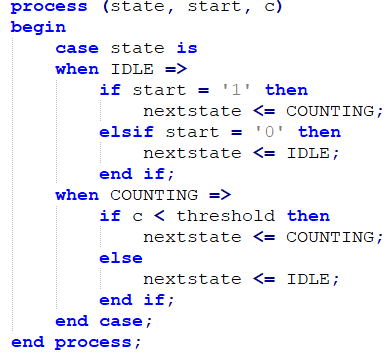
\includegraphics[scale=0.6]{nextState.PNG}
\caption{Process \#1}
\end{figure}

\subsubsection{Vérification du code}

\subparagraph{Sensitity list}
	Tout les éléments pris en compte pour le calcul de l'état suivant sont : State, start et c. Alors la liste dois être (state, start,c).
	
\subparagraph{Calcul des états}
	Si l'on regarde le dessin de l'automate fournis : 
\begin{itemize}
\item Dans l'état IDLE on reste dans cet état si start vaut '0', sinon si start vaux '1' on vas dans l'état COUNTING. Ce qui est exprimé dans ce code
\item Dans l'état COUNTING on reste dans cet état si c est < à treshold, sinon on vas dans l'état IDLE. Ce qui est aussi exprimé dans ce code.
\end{itemize}



\newpage	

\subsection{Mise à jour de l'état}

	D'après les slide, ce process exprime la mise à jour de la valeur du registre courrant en synchronisation avec l'horloge. Ce process peux aussi prendre en considération le signal "reset".
	
\subsubsection{Le code}

Après avoir modifier le code tel que : 
\begin{figure}[!h]
\advance\leftskip-0.4cm
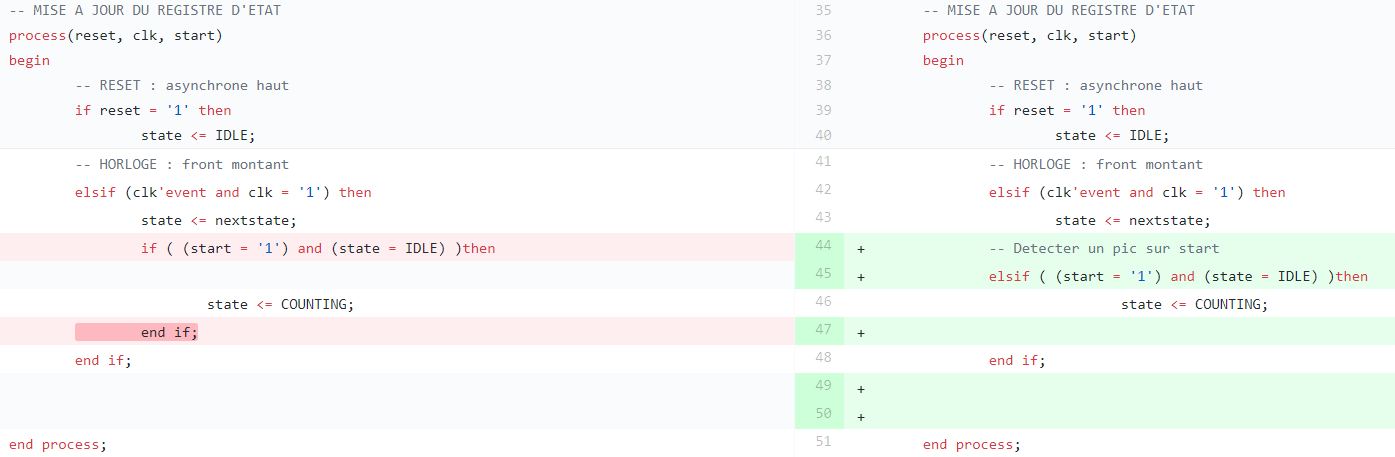
\includegraphics[scale=0.6]{oldProc1.PNG}
\caption{Process \#2 Avant/après }
\end{figure}

\subsubsection{Vérification du code}
\subparagraph{Sensitity list}
	Tout les éléments pris en compte pour le calcul de l'état suivant sont : reset clock et start. Je prend en compte ici start car je veux que la moindre impulsion sur le signal start puisse déclancher le compte à rebours et que pas uniquement lorsque l'horloge est sur un front montant. Je suis donc obligé de l'écrire ici.
Néanmoins, j'avais fais une erreur d'imbrication de if/elsif précédement.	
\subparagraph{Reset} Il y a bien une mise à de l'état courrant si le reset est à sur un 1 (asynchronous reset HIGH)

\subparagraph{Front montant}
L'état ce met bien à jour si l'on se trouve sur un front montant de l'horloge.


	
\subsection{Mise à jour de du compteur}

	Il n'y as pas d'indication dans le cours pour implémenter le counter mais d'après moi il faut un process qui s'en occupe.
	

\subsubsection{Le code}

Après avoir modifier le code tel que : 
\begin{figure}[!h]
\advance\leftskip-0.4cm
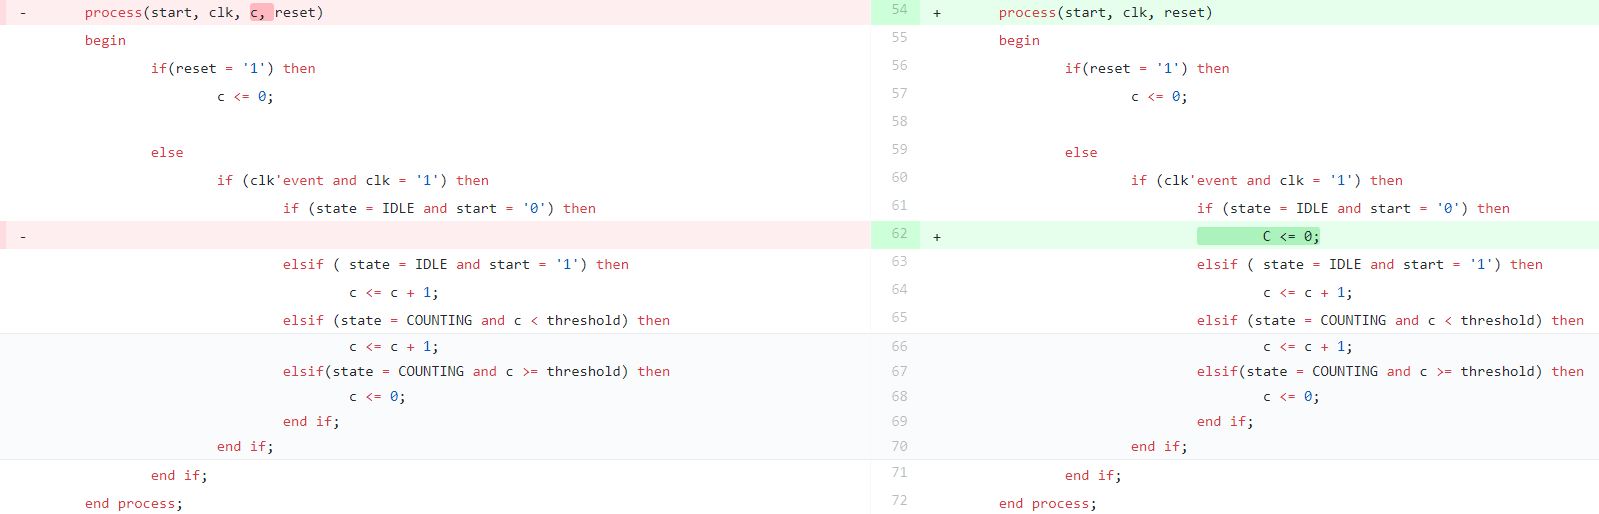
\includegraphics[scale=0.55]{oldProc2.PNG}
\caption{Process \#3 Avant/après }
\end{figure}

\newpage


J'avais "juste" oublié une ligne de code et un signal en trop dans la liste de senssibilité. C'est comme ça qu'une fusée peux exploser...
 
\subsubsection{Vérification du code}
\subparagraph{Sensitity list} La valeur de c peux changer si et seulement si soit start, clk et reset d'ou la list (start, clk, reset). 
	
	


\subparagraph{Transitions}
J'ai retranscris les transitions de l'automate tel que les calculs de c ne se fasse uniquement une fois par cycle.  



\subsection{Exprime les fonctions de sorties}

D'après les slides il faut un process qui exprime les fonctions de sorties (ou un ensemble de concurent statement)

\subsubsection{Le code}

J'avais exprimé cela sous la forme :
\begin{verbatim}
aboveth <= '0' when c < threshold else '1';
\end{verbatim}

car je n'ai pas réussi à trouver la comparaison bouléenne exprimant $\geq$ 

Pour être sur de moi, j'ai transformé le tout en un process :

\begin{figure}[!h]
\advance\leftskip+2cm
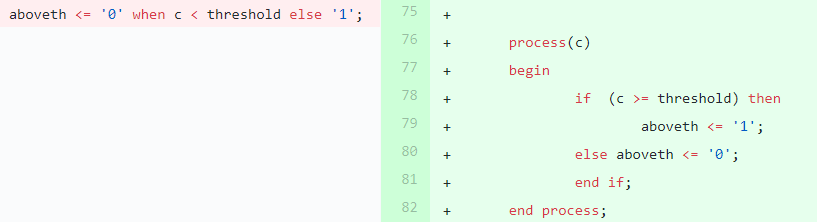
\includegraphics[scale=0.7]{oldProc3.PNG}
\caption{Process \#4 Avant/après }
\end{figure}

\subsubsection{Vérification du code}
	Je pense pas qu'il n'y ai vraiment grand chose à commenter.

\section{Improve testbench for the system.}
Il faut déjà changé le testbench avec la vrai valeur de l'horloge, je n'ai pas vraiment le temps de le faire...
\end{document}